% \textbf{how do we determine the overall membership}
% relevant info of the membership is in M11 table 1
% cannot determine the membership of two galaxies 
% spatial cut is defined in M11 p.9 first paragraph 

% paragraphs needs to be reorganized 
The overall membership of the galaxies
of El Gordo was first determined using a shifting gapper method
\citep{Fadda96} after applying a rest frame cut of
4000~\kilo\meter~\second$^{-1}$ \citep{Sifon13}. This method gives a
total count of 89 galaxy members of El Gordo.
To further distinguish member galaxies of each subcluster, we adopt a spatial cut approximately perpendicular to the 2D merger axis
from \citepalias{M11}. Using this cut, we determined that there are 54
members in the NW subclusters and 35 members in the SE subclusters (See Figure
\ref{fig:membership}). The spatial cut indicated by the green line was done after
mapping the world coordinates to pixel coordinates to avoid anamorphic distortion. 
Then, we bootstrapped the biweight locations of the redshifts of the
respective members in order to obtain the PDFs of the redshifts of each
subcluster 
\citep{Sifon13}. Using this method of determining subcluster members, the spectroscopic
redshift of the subclusters were determined to be $z_{NW} = 0.86901 \pm
0.00017$ and $z_{SE} = 0.87175 \pm 0.00019$, where the quoted numbers represent the biweight location and
biweight scale respectively \citep{Beers90}. 
These biweight location
estimators are less susceptible to outliers than the mean and standard
deviations. These redshifts of the subclusters correspond to a relative
velocity difference of $476$ km/s. 

\begin{figure}
	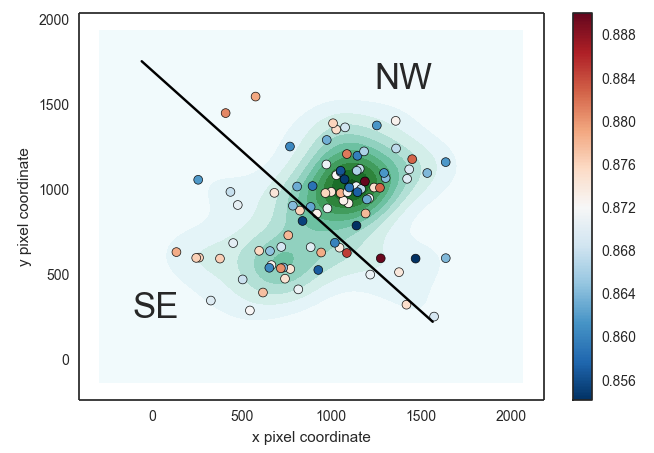
\includegraphics[width = \linewidth]{confirmed_member_divide.png}
	\caption{\label{fig:membership} The division of
the member galaxies among the two subclusters of El Gordo by a spatial cut
(green line). The color bar shows the color mapping of the spectroscopic
redshift of the member galaxies, with the redder end indicating higher
redshift.} 
\end{figure}

%We confirm the existence of the subclusters of El Gordo from the 2D spatial
%location of the galaxies, with the more massive cluster lying in the
%northwest (NW) and the less massive subcluster lying in the southeast(SE)  (REF - also have to reference the other literature
%for confirmation in the other wavelengths)
%
%Specifically, the membership of the NW and SE subclusters are
%determined based on a combination of the redshift and the spatial location. 
